\appendix

\section{Uptime patterns}

\begin{figure*}[t]
	\centering
	
\includegraphics[width=\textwidth]{diagrams/heartbleed-uptimes.jpg}
	\caption{April 2014, the month the Heartbleed bug was discovered.  The Tor
		Project asked relay operators to change their keypairs.  As a result,
		our tool flagged many relays as disappearing and appearing at the same
		time.  The large block in the middle of the diagram happened because The
		Tor Project eventually rejected a large number of relays that did not
		change their keypairs in time.}
	\label{fig:heartbleed-uptimes}
\end{figure*}

\begin{figure*}[t]
	\centering
	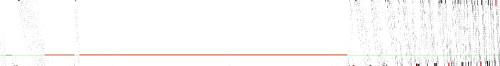
\includegraphics[width=\textwidth]{diagrams/lizard-uptimes.jpg}
	\caption{December 2014, when a group of people started several hundred Tor
	relays in the Google cloud.  The relays were only online for a small number
	of hours because they were promptly rejected by The Tor Project.}
	\label{fig:lizard-uptimes}
\end{figure*}

\begin{figure*}[t]
	\centering
	
\includegraphics[width=\textwidth]{diagrams/planetlab-uptimes.jpg}
	\caption{December 2014, when a group of people started several hundred Tor
	relays in the Google cloud.  The relays were only online for a small number
	of hours because they were promptly rejected by The Tor Project.}
	\label{fig:lizard-uptimes}
\end{figure*}

\section{Reproducing our work}
% \begin{lstlisting}
% go get git.torproject.org/user/phw/sybilhunter.git
% \end{lstlisting}
Redacted for anonymization.

\section{Mathematical metric}
\label{sec:metric}
The following conditions have to be met in order to classify as a mathematical
metric.  While points 1, 2, and 3 are typically straightforward to satisfy,
point 4, the triangle inequality, can turn out to be tricky.
\begin{enumerate}
	\item $d(x, y) \geq 0$
	\item $d(x, y) = 0$ iff $x = y$
	\item $d(x, y) = d(y, x)$
	\item $d(x, z) \leq d(x, y) + d(y, z)$
\end{enumerate}
